\clearpage
\expchapter{实验四\quad 翻转的花朵}
\sect{教学目标}
\noindent\hspace*{2em}关键词：数组，位图，灰度图像，像素矩阵\par
\noindent\hspace*{2em}知识和能力目标：理解和熟练掌握多维数组的存储及其操作方法，本例主要是对 BMP 位图文件的像素矩阵进行操作。\par
\noindent\hspace*{2em}价值目标：\par
\noindent\hspace*{2em}科学精神：一幅图像，一篇文章，一个社交关系网络，都可以抽象为一个关系矩阵。由此，我们可以将翻转图像、计算文章相似度、找到社交网络中的大 V，统一为对矩阵的计算问题。\par
\noindent\textbf{工程观：}\par
\noindent\hspace*{2em}如果有人说，在我们的生活和工作中，数学无处不在，你会如何回应？\par
\sect{问题描述}
\noindent\hspace*{2em}数字图像数据可以用矩阵来表示，因此可以用矩阵理论和矩阵算法对数字图像进行分析和处理。以灰度图像\footnote{灰度图像是一种具有从黑到白 256 级灰度色域或等级的单色图像。该图像中的每个像素用 8 位数据表示，因此像素点值介于黑白间的 256 种灰度中的一种。该图像只有灰度等级，而没有颜色的变化。}为例（图 1）。灰度图像的像素数据就是一个矩阵，矩阵的行对应图像的高（单位为像素），矩阵的列对应图像的宽，矩阵元素对应图像的像素，矩阵元素的值就是像素的灰度值。\par
\begin{center}

\includegraphics[width=0.5\textwidth]{images/exp4-1.png}
\end{center}
\figcaption{图 1 图像像素矩阵}
\noindent\hspace*{2em}BMP 是一种与硬件设备无关的图像文件格式，采用位映射存储格式。BMP 图像的深度有 1bit（2色）、4bit（16 色）、8bit（256 色）及 24bit（真彩色）。BMP 文件存储位图数据时，图像扫描方式是：在行内按从左到右扫描、在行间从下到上扫描的顺序。Windows 规定图像文件中，一个图像的扫描行所占的字节数必须是 4 的倍数，不足的以 0 填充。\par
\noindent\hspace*{2em}biWidth：图像的宽度，单位是像素\par
\noindent\hspace*{2em}biBitCount：每个像素所需位数，常用 1bit（2 色）、4bit（16 色）、8bit（256 色）、24bit（真彩色）。如果 biBitCount = 8，1 个像素 8bit，1 个像素占 1 字节；如果 biBitCount = 24，1 个像素 24bit，1 个像素占 3 字节。\par
\noindent\hspace*{2em}对 BMP 图像，要求是 4 字节对齐，即每行字节数必须为 4 的整数倍，因此满足以 4 字节为对齐单位向下对齐，所以每行字节数为：\par
\noindent\hspace*{2em}\texttt{PerLineBytes = (((biWidth * biBitCount) / 8 + 3) / 4) * 4}\par
\noindent\hspace*{2em}图像的镜像（mirror）分水平镜像和垂直镜像两种，图像的转置可看成是逆时针旋转 90 度。以下是一幅图像的原图、水平镜像、垂直镜像和转置图像（示意图）。\par
\begin{center}
\begin{minipage}{0.22\textwidth}
\centering

\includegraphics[width=\linewidth]{images/exp4-2.png}\\
{\small 原图}
\end{minipage}\hfill
\begin{minipage}{0.22\textwidth}
\centering
\scalebox{-1}[1]{
\includegraphics[width=\linewidth]{images/exp4-2.png}}\\
{\small 水平镜像}
\end{minipage}\hfill
\begin{minipage}{0.22\textwidth}
\centering
\scalebox{1}[-1]{
\includegraphics[width=\linewidth]{images/exp4-2.png}}\\
{\small 垂直镜像}
\end{minipage}\hfill
\begin{minipage}{0.22\textwidth}
\centering
\rotatebox{90}{
\includegraphics[width=\linewidth]{images/exp4-2.png}}\\
{\small 转置}
\end{minipage}
\end{center}

\noindent\hspace*{2em}本问题的任务是：编写程序，对任意 \textbf{BMP }图像，将其水平镜像、垂直镜像、转置，将处理后的图像保存到文件。假设如下：为简化问题，图像为 256 色 BMP 图，也可尝试操作 2 色、16 色、24 位真彩色 BMP 图。\par
\sect{基本思路}
\noindent\hspace*{2em}读取 BMP 图像：一个 BMP 文件的存储形式如下：\par
\begin{center}

\includegraphics[width=0.85\textwidth]{images/exp4-3.png}
\end{center}

\noindent\hspace*{2em}主要由以下四部分构成，因此读取一幅 \textbf{256} 色 \textbf{BMP }图像时，需分别读取以上四部分信息，存盘也要保存这四部分信息。第 4 部分为我们实际要处理（镜像和转置）的像素数据：位图全部的像素，是按自下向上，自左向右的顺序排列的。\par
\begin{center}
\fontsize{8.5pt}{11pt}\selectfont
\renewcommand{\arraystretch}{1.12}
\begin{tabular}{|c|l|p{6cm}|}
\hline
1 & 位图文件头 BITMAPFILEHEADER & 文件头结构，14 字节 \\ \hline
2 & 位图信息头 BITMAPINFOHEADER & 信息头结构，40 字节 \\ \hline
3 & 调色板 Palette & 256 色 BMP 含 256 项 RGBQUAD（1024 字节） \\ \hline
4 & 实际的位图数据 ImageData & 256 色 BMP 每像素 1 字节 \\ \hline
\end{tabular}
\end{center}
\noindent\hspace*{2em}本次实验将 BMP 像素数据加载到 Rust 的 \texttt{Vec<Vec<u8>>}，约定 \texttt{pixels[row][col]} 表示第 \texttt{row} 行、第 \texttt{col} 列像素，行号 0 为图像顶行。BMP 文件在磁盘上是"自下而上"存储的，这一层转换在 \texttt{read\_pixels}/\texttt{write\_pixels} 内部完成，对外屏蔽。\par
\noindent\hspace*{2em}\textbf{三种变换的位置计算公式：}\par
\noindent\hspace*{2em}设原图宽 $w$、高 $h$，坐标 $(i, j)$ 表示第 $i$ 行第 $j$ 列（$0 \le i < h$，$0 \le j < w$）。\par
\noindent\hspace*{2em}（1）水平镜像（mirror\_h）：同一行内左右翻转，$(i, j) \to (i, w-1-j)$，宽高均不变。\par
\noindent\hspace*{2em}（2）垂直镜像（mirror\_v）：行间上下翻转，$(i, j) \to (h-1-i, j)$，宽高均不变。\par
\noindent\hspace*{2em}（3）转置（transpose）：行列互换，$(i, j) \to (j, i)$，新图宽 $h$、新高 $w$。\par
\noindent\hspace*{2em}对 24 位真彩色 BMP，读入时按 BT.601 加权灰度 $Y = 0.299R + 0.587G + 0.114B$ 量化到 8 位灰度，输出时构造一份 256 项灰度调色板，从而统一在 8 位灰度 BMP 域中处理。\par
\sect{实验结果及分析}
\noindent\hspace*{2em}1. 实验结果\par
\noindent\hspace*{2em}（1）实验过程描述\par
\noindent\hspace*{2em}1. 本实验用 Rust 语言开发，使用 Cargo 构建系统和 rustc 编译器，运行机器为本人笔记本电脑（macOS，Apple Silicon）。本人独立完成编码和测试，参考 BMP 文件格式相关资料实现 \texttt{FileHeader}/\texttt{InfoHeader}/\texttt{RgbQuad} 的字节布局。\par
\noindent\hspace*{2em}2. 测试数据选取思路为：典型、覆盖不同图像内容、覆盖不同位深度。共选取 4 张输入图像：(a) \texttt{flower.bmp}，48$\times$32 灰度 256 色 BMP，模拟一朵不对称花朵，便于观察镜像差异；(b) \texttt{gradient.bmp}，48$\times$32 灰度 256 色 BMP，左暗右亮的水平灰度渐变；(c) \texttt{stripes.bmp}，48$\times$32 灰度 256 色 BMP，垂直黑白相间条纹；(d) \texttt{flower\_real.bmp}，242$\times$160 的 24 位真彩色花朵照片（外部导入并经过程序自动量化，文件高度为负时按顶向下顺序读取）。\par
\noindent\hspace*{2em}3. 三种变换的正确性、对合性以及文件往返后像素值是否完全保留是测试重点。水平镜像和垂直镜像连续做两次应当回到原图；转置后宽高交换；行 4 字节对齐在 \texttt{line\_bytes} 中已统一处理。\par
\noindent\hspace*{2em}（2）测试结果\par
\noindent\hspace*{2em}运行实验程序对 4 张输入图分别做水平镜像、垂直镜像和转置，得到 12 张结果图。\par
\noindent\hspace*{2em}首先是 \texttt{flower.bmp}（花朵，48$\times$32 灰度 256 色）：\par
\begin{center}
\begin{minipage}{0.22\textwidth}
\centering

\includegraphics[width=\linewidth]{images/exp4-1.png}\\
{\small 原图 (48$\times$32)}
\end{minipage}\hfill
\begin{minipage}{0.22\textwidth}
\centering

\includegraphics[width=\linewidth]{images/exp4-2.png}\\
{\small 水平镜像}
\end{minipage}\hfill
\begin{minipage}{0.22\textwidth}
\centering

\includegraphics[width=\linewidth]{images/exp4-3.png}\\
{\small 垂直镜像}
\end{minipage}\hfill
\begin{minipage}{0.22\textwidth}
\centering

\includegraphics[width=\linewidth]{images/exp4-4.png}\\
{\small 转置 (32$\times$48)}
\end{minipage}
\end{center}

\noindent\hspace*{2em}可以看到，转置后图幅从 48$\times$32 变成 32$\times$48，符合"行列互换"的预期。\par
\noindent\hspace*{2em}其次是 \texttt{gradient.bmp}（2D 灰度渐变，左上角最亮、向右下方向单调变暗）。\par
\begin{center}
\begin{minipage}{0.30\textwidth}
\centering

\includegraphics[width=\linewidth]{images/exp4-5.png}\\
{\small 原图}
\end{minipage}\hfill
\begin{minipage}{0.30\textwidth}
\centering

\includegraphics[width=\linewidth]{images/exp4-6.png}\\
{\small 水平镜像}
\end{minipage}\hfill
\begin{minipage}{0.30\textwidth}
\centering

\includegraphics[width=\linewidth]{images/exp4-7.png}\\
{\small 垂直镜像}
\end{minipage}
\end{center}

\noindent\hspace*{2em}水平镜像后，亮暗方向反转（左上亮变成右上亮）；垂直镜像后，顶行底行互换（左上亮变成左下亮），与原图差异明显。\par
\noindent\hspace*{2em}再观察 \texttt{stripes.bmp}（垂直条纹）：\par
\begin{center}
\begin{minipage}{0.30\textwidth}
\centering

\includegraphics[width=\linewidth]{images/exp4-9.png}\\
{\small 原图：垂直黑白条纹}
\end{minipage}\hfill
\begin{minipage}{0.30\textwidth}
\centering

\includegraphics[width=\linewidth]{images/exp4-10.png}\\
{\small 水平镜像：条纹镜像翻转}
\end{minipage}\hfill
\begin{minipage}{0.30\textwidth}
\centering

\includegraphics[width=\linewidth]{images/exp4-11.png}\\
{\small 垂直镜像：与原图相同}
\end{minipage}
\end{center}

\noindent\hspace*{2em}对行内无差异的图像（如纯垂直条纹），垂直镜像结果与原图相同，验证了算法对此类特殊情形的正确性。\par
\noindent\hspace*{2em}最后是一张 24 位真彩色照片 \texttt{flower\_real.bmp}（242$\times$160），经过程序自动量化为 8 位灰度后做三种变换：\par
\begin{center}
\begin{minipage}{0.22\textwidth}
\centering
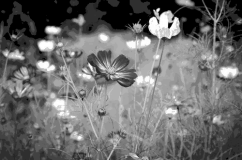
\includegraphics[width=\linewidth]{images/exp4-orig.png}\\
{\small 原图 (242$\times$160)}
\end{minipage}\hfill
\begin{minipage}{0.22\textwidth}
\centering
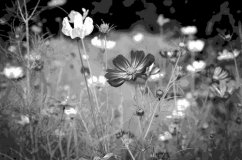
\includegraphics[width=\linewidth]{images/exp4-rh.png}\\
{\small 水平镜像}
\end{minipage}\hfill
\begin{minipage}{0.22\textwidth}
\centering
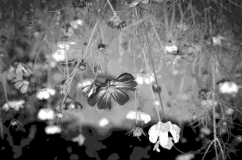
\includegraphics[width=\linewidth]{images/exp4-rv.png}\\
{\small 垂直镜像}
\end{minipage}\hfill
\begin{minipage}{0.22\textwidth}
\centering
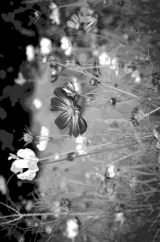
\includegraphics[width=\linewidth]{images/exp4-rt.png}\\
{\small 转置 (160$\times$242)}
\end{minipage}
\end{center}

\noindent\hspace*{2em}转置结果尺寸 160$\times$242 与原图宽高互换一致，证明变换后 \texttt{biWidth}/\texttt{biHeight}/\texttt{biSizeImage} 三个信息头字段均被同步更新。\par
\noindent\hspace*{2em}用 \texttt{cargo test} 运行的 5 个模块测试和 14 个集成测试全部通过，覆盖：BMP 字节级往返、对合性（变换两次回到原图）、行列互换、各种行字节对齐（3 像素宽自然产生 4 字节对齐行）、24 位真彩色读取与量化、负高度 BMP 顶向下读取、单文件输出目录创建、目录批量处理等。\par
\noindent\hspace*{2em}4. 实验方案分析\par
\noindent\hspace*{2em}（1）本实验设计的优点，不足，时空开销等问题分析\par
\noindent\hspace*{2em}\textbf{优点：}\par
\noindent\hspace*{2em}1. 像素矩阵采用 \texttt{Vec<Vec<u8>>} 抽象，水平镜像、垂直镜像、转置三种算法均写为行/列映射的纯函数，无副作用。\par
\noindent\hspace*{2em}2. BMP 文件的"自下而上"扫描与内存矩阵的"自上而下"约定在 \texttt{read\_pixels}/\texttt{write\_pixels} 内部完成，对上层算法完全透明。\par
\noindent\hspace*{2em}3. 支持 8 位带调色板 BMP 与 24 位真彩色 BMP 两种主流格式；24 位输入时按 BT.601 加权灰度量化到 8 位灰度 BMP 输出，免去对 24 位像素数据直接做行存储的开销。\par
\noindent\hspace*{2em}4. 4 字节对齐在 \texttt{line\_bytes} 一处集中计算，单元测试覆盖了"3 像素宽必为 4 字节对齐行"等关键边界。\par
\noindent\hspace*{2em}\textbf{不足与时空开销：}\par
\noindent\hspace*{2em}1. 内存占用为 $O(w \cdot h)$ 字节，对于极大图像（如 4K 真彩色照片）会一次性占用 $O(w \cdot h \cdot 3)$；本实验暂未实现分块流式处理。\par
\noindent\hspace*{2em}2. 转置算法需重新分配一个新矩阵，复杂度 $O(w \cdot h)$，无可避免；如追求零分配，可借助原地置换，但会显著增加代码复杂度，得不偿失。\par
\noindent\hspace*{2em}3. 当前实现仅支持 8 位和 24 位 BMP，未实现 1 位/4 位带调色板 BMP 的读取（这需要在像素索引到调色板之间再增加一层 1bit/2bit 解包）。\par
\noindent\hspace*{2em}4. 24 位 BMP 量化时会丢失色彩信息；对色彩敏感的图像建议改用"读 24 位、写 24 位"模式，仅在内存中加灰度视图。\par
\noindent\hspace*{2em}5. 附件：源程序代码\par
{\fontsize{6pt}{8pt}\selectfont
\setlength{\parindent}{0pt}
\begin{multicols}{2}
\begin{verbatim}
// Cargo.toml
[package]
name = "ec_exp_4"
version = "0.1.0"
edition = "2021"

[lib]
name = "exp_4"

// src/lib.rs
pub mod bmp;
pub mod image;

pub use bmp::{build_bytes, line_bytes,
    read_file, read_pixels, write_file,
    FileHeader, InfoHeader, RgbQuad};
pub use image::{process_dir,
    process_file, Image};

// src/image.rs（节选）
pub fn process_file<P: AsRef<Path>,
    Q: AsRef<Path>>(
    input: P, out_dir: Q
) -> io::Result<()> {
    fs::create_dir_all(&out_dir)?;
    let img = Image::read(&input)?;
    let input_name = input.as_ref()
        .file_stem()
        .and_then(|s| s.to_str())
        .unwrap_or("image")
        .to_string();

    img.mirror_horizontal().write(
        out_dir.as_ref().join(format!(
            "{}_mirror_h.bmp", input_name)))?;
    img.mirror_vertical().write(
        out_dir.as_ref().join(format!(
            "{}_mirror_v.bmp", input_name)))?;
    img.transpose().write(
        out_dir.as_ref().join(format!(
            "{}_transpose.bmp", input_name)))?;
    Ok(())
}
\end{verbatim}

\columnbreak

\begin{verbatim}
// src/bmp.rs
use std::fs;
use std::io;
use std::path::Path;

#[derive(Clone, Debug)]
pub struct FileHeader {
    pub bf_type: [u8; 2],
    pub bf_size: u32,
    pub bf_reserved1: u16,
    pub bf_reserved2: u16,
    pub bf_off_bits: u32,
}

#[derive(Clone, Debug)]
pub struct InfoHeader {
    pub bi_size: u32,
    pub bi_width: i32,
    pub bi_height: i32,
    pub bi_planes: u16,
    pub bi_bit_count: u16,
    pub bi_compression: u32,
    pub bi_size_image: u32,
    pub bi_x_pels_per_meter: i32,
    pub bi_y_pels_per_meter: i32,
    pub bi_clr_used: u32,
    pub bi_clr_important: u32,
}

pub fn line_bytes(width: u32,
    bit_count: u16) -> u32 {
    ((width * bit_count as u32 + 31) / 32) * 4
}

pub fn read_pixels(buf: &[u8], off: usize,
    width: u32, height: u32,
    bit_count: u16, top_down: bool
) -> Vec<Vec<u8>> {
    let lb = line_bytes(width, bit_count) as usize;
    let mut mat = vec![
        vec![0u8; width as usize];
        height as usize
    ];
    for row in 0..height as usize {
        let bmp_row = if top_down {
            row
        } else {
            height as usize - 1 - row
        };
        let line_start = off + bmp_row * lb;
        for col in 0..width as usize {
            mat[row][col] = buf[line_start + col];
        }
    }
    mat
}

pub fn quantize_to_gray(
    rgb: &[Vec<(u8, u8, u8)>]
) -> Vec<Vec<u8>> {
    rgb.iter().map(|row| row.iter()
        .map(|&(r, g, b)| {
            ((299 * r as u32 + 587 * g as u32
                + 114 * b as u32) / 1000) as u8
        })
        .collect())
        .collect()
}
\end{verbatim}
\end{multicols}
}

{\fontsize{6pt}{8pt}\selectfont
\setlength{\parindent}{0pt}
\noindent\textbf{测试用例}\par
\noindent (a) 8 位 BMP 字节级往返：写出 4$\times$2 矩阵（含调色板），再读回，像素值完全一致。\par
\noindent (b) 水平镜像对合性：$4\times2$ 矩阵镜像两次回到原值。\par
\noindent (c) 垂直镜像对合性：$4\times2$ 矩阵垂直镜像两次回到原值。\par
\noindent (d) 转置对合性：$4\times2$ 矩阵转置两次回到原值。\par
\noindent (e) 转置行列互换：$3\times2$ 矩阵转置后宽高变为 2$\times$3，像素 $(i,j) \to (j,i)$。\par
\noindent (f) 文件往返：临时目录创建 2$\times$3 BMP，转置后写出再读回，$3\times2$ 像素矩阵完全一致。\par
\noindent (g) 行字节对齐：3 像素宽 8 位 BMP 每行 4 字节，2 行共 8 字节。\par
\noindent (h) 24 位 BMP 量化：构造 2$\times$2 的 24 位 BMP（蓝/白/红/绿），读入后调色板为 256 项灰度，灰度值与 BT.601 期望一致。\par
\noindent (i) 负高度 BMP 读取：构造顶向下存储的 24 位 BMP，读入后顶行和底行顺序保持正确。\par
\noindent (j) 转置更新信息头：转置后 \texttt{biWidth} 与 \texttt{biHeight} 已交换。\par
\noindent (k) 单文件处理：单文件 3 变换输出共 3 个 .bmp，且输出目录不存在时可自动创建。\par
\noindent (l) 目录处理：含 5 个 .bmp 的目录，输出 15 个 .bmp。\par
}
